\section{Drag on the actuator disks}
%kommenter at me uansett bryr oss mest om 10m/s, som e i den stabile delen 

The drag coefficient on the produced ADs has been studied. Initially, the solid disk, used as a reference case, produced the drag seen in figure \ref{Fig:SolidDrag} and the drag coefficient seen in figure \ref{Fig:SolidCD}. Further, the drag and the drag coefficient for the two types of disks with 60\% solidity can be seen in figure \ref{Fig:SixtyDrag} and \ref{Fig:SixtyCD}, respectively. For all three disks, the drag is seen to increase with increasing wind velocity, as one would expect. The average drag coefficient and the standard deviation is presented in table \ref{tab:AvgCD}.


\begin{figure} [h!]
    \centering
    \begin{subfigure}[b]{0.45\linewidth}
        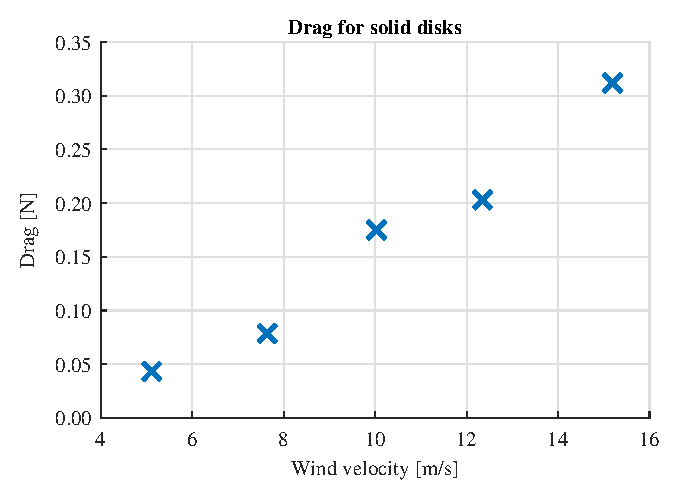
\includegraphics[width=\textwidth]{0_Images/SolidDrag.eps}
        \caption{The drag.}
        \label{Fig:SolidDrag}
    \end{subfigure}
    ~
    \begin{subfigure}[b]{0.45\linewidth}
        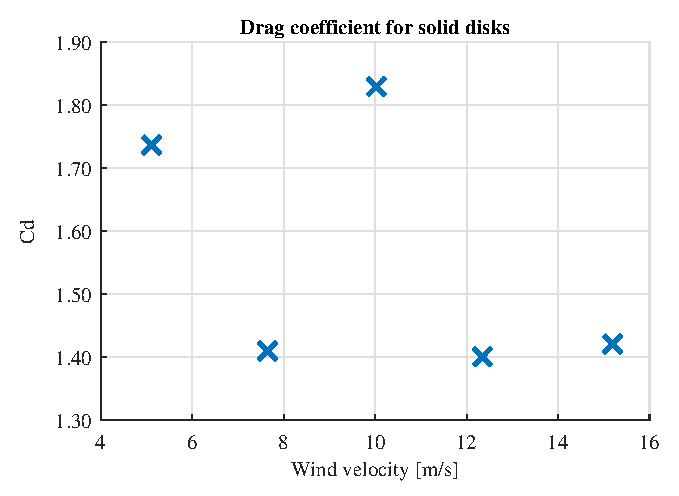
\includegraphics[width=\textwidth]{0_Images/SolidCD.eps}
        \caption{The drag coefficient.}
        \label{Fig:SolidCD}
    \end{subfigure}
    \caption{Using the solid disk.}
    \label{fig:SolidDisk}
\end{figure}


\begin{figure} [h!]
    \centering
    \begin{subfigure}[b]{0.45\linewidth}
        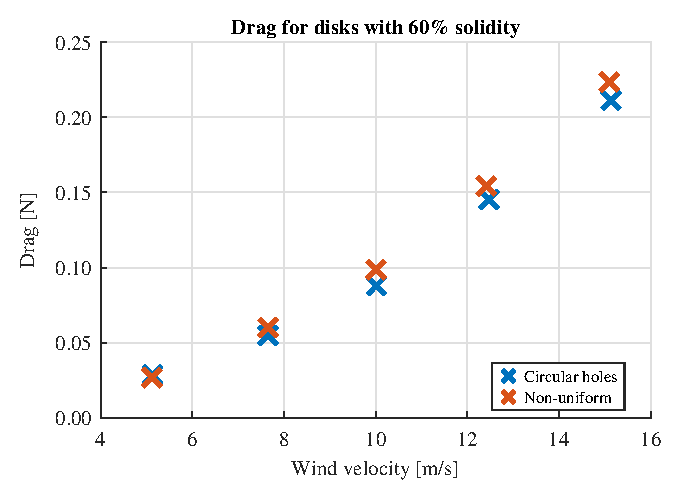
\includegraphics[width=\textwidth]{0_Images/SixtyDrag.eps}
        \caption{The drag.}
        \label{Fig:SixtyDrag}
    \end{subfigure}
    ~
    \begin{subfigure}[b]{0.45\linewidth}
        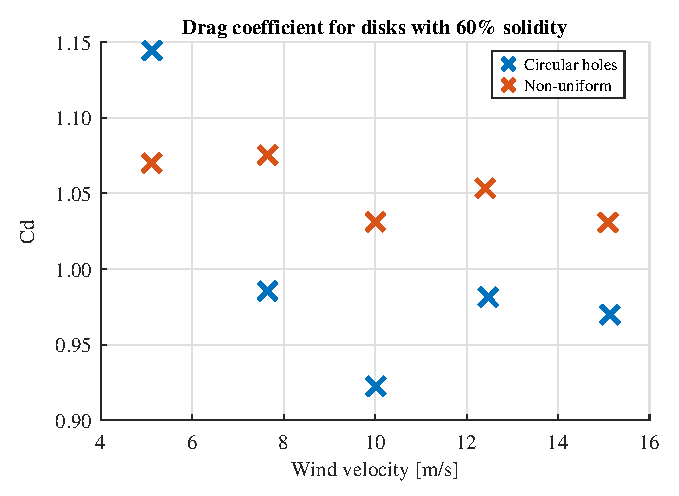
\includegraphics[width=\textwidth]{0_Images/SixtyCD.eps}
        \caption{The drag coefficient.}
        \label{Fig:SixtyCD}
    \end{subfigure}
    \caption{Using the disks with 60\% solidity.}
    \label{fig:SixtyDisk}
\end{figure}

\FloatBarrier

Further, the drag and drag coefficient for the disks with 40\% and 35\% solidity were plotted in figure \ref{fig:FortyDrag} and \ref{fig:FortyCD}. As these disks produced a drag coefficient fairly close to the average drag coefficient of the rotating turbines, this value is also included in the plots. The average drag coefficient and standard deviation can be seen in table \ref{tab:AvgCD}. 

\begin{figure}[h!]
    \centering
    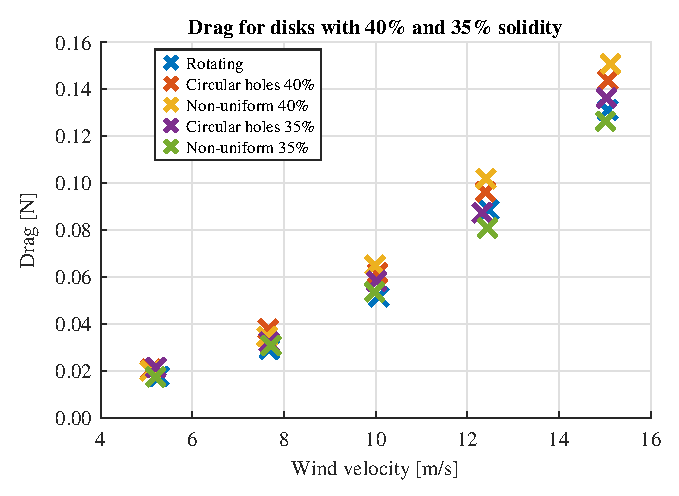
\includegraphics[width=\linewidth]{0_Images/FortyDrag.eps}
    \caption{The drag for the disks with 40\% and 35\% solidity, compared to the average drag coefficient of the rotating disks.}
    \label{fig:FortyDrag}
\end{figure}

\begin{figure}[h!]
    \centering
    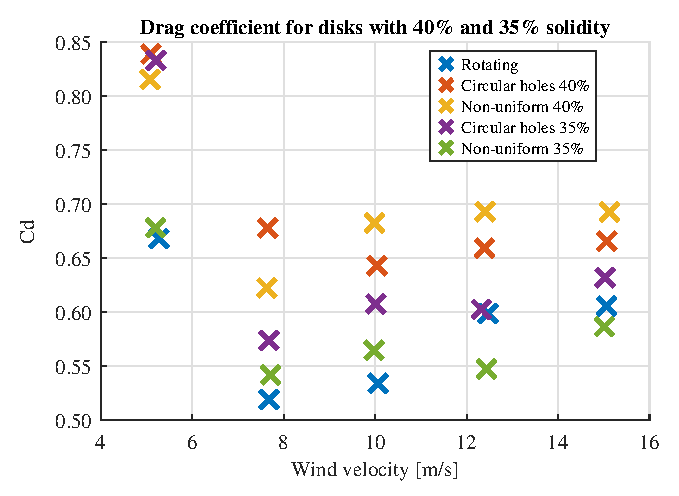
\includegraphics[width=\linewidth]{0_Images/FortyCD.eps}
    \caption{The drag coefficient for the disks with 40\% and 35\% solidity, compared to the average drag coefficient of the rotating disks.}
    \label{fig:FortyCD}
\end{figure}


Some general trends can be observed. For all disks presented in figure \ref{fig:FortyCD}, as well as for the disk with circular holes at 60\% solidity in figure \ref{Fig:SixtyCD}, Cd measured at 5 m/s is significantly higher than for the other velocities, while the measurements at the four other velocities seem to concentrate around some mean value. This may be a result of ... 


\begin{table}[H]
    \centering
    \begin{tabular}{l c c r}
         Disk type & Average Cd & SD \\
         \hline
         Rotating average & 0.601 & 0.080 \\
         Solid & 1.515 & 0.207 \\
         Uniform holes, 60\% & 0.965 & 0.084 \\
         Non-uniform, 60\% & 1.048 & 0.021 \\
         Uniform holes, 40\% & 0.697 & 0.080 \\
         Non-uniform, 40\% & 0.701 & 0.070 \\
         Uniform holes, 35\% & 0.650 & 0.104 \\
         Non-uniform, 35\% & 0.584 & 0.056 \\
    \end{tabular}
    \caption{Average Cd for each disk.}
    \label{tab:AvgCD}
\end{table}

%for last one, 0.5843 without drift 

In terms of these results, the non-uniform disk can be seen to produce a slightly higher drag at the same solidity compared to the uniform disk at 60\% and 40\% solidity. The same trend can not be seen at 35\% solidity, however this design with holes is created in a different way, with a larger circumference, and may not be exactly comparable. The non-uniform 35\% disk seems to best match the rotating WT model. 

As can readily be seen, the drag coefficient decreases with decreasing solidity, as one would expect. This can be compared to \cite{Lignarolo2016}, who presented a comparison between different drag coefficients as a function of solidity as presented in six different studies found in literature. According to this, a solidity of 60\% results in a Cd of around 0.9, a solidity of 40\% results in a Cd between 0.5 and 0.6, and a 35\% solidity results in a Cd between 0.4 and 0.5. Compared, the disks used in this study presents a higher drag for all solidities. This can be caused by conditions such as inflow turbulence. 

%Which SD is relevant? I have the ones for each measurement... But maybe the ones for Cd also? 

%\section{Noise and other possible sources of error}

%\begin{figure}[h!]
%    \centering
%    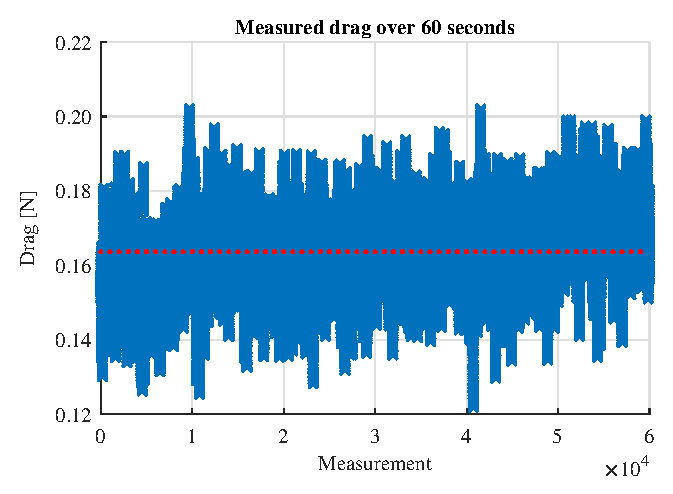
\includegraphics[width=\linewidth]{0_Images/NoiseFirst.eps}
%    \caption{The drag for the solid disk at 5 m/s.}
%    \label{fig:Noise}
%\end{figure}

%Figure \ref{fig:Noise} shows each measured drag value at a sampling rate of 1000 Hz over the course of 60 seconds. The measured drag varies with a 0.012, compared to an average of 0.1636. This means that the noise is of one order less that the average. 

This noise may both be related to measurement noise in the force plate, and electrical noise as the signal passes from the force plate, through the amplifier and the lowpass filter. It is still a reasonable assumption that the measurements have a Gaussian distribution and that the average drag is representative. 

The measured temperature only varies between about 20\degree C and 23\degree C. Since this variation is fairly small, it is assumed to not have any significant impact on the resulting drag. 



%Error, standard deviation 

%why do we get the results that we get? 

%- Adjusting for drift 
%- statistikk arument 
%- usikkerhet



